\subsection{一致连续函数的延拓}

当所讨论的函数取值于完备豪斯多夫一致空间时，连续延拓定理（第一章 § 8 第 5 目定理 1）有重要的补充。

命题 11 设 A 是拓扑空间 X 的稠密子集，并设 f 是 A 到完备豪斯多夫一致空间 X' 中的一个映射。则 f 可由连续性延拓到 X，当且仅当对每个 x ∈ X，x 在 X 中的邻域滤子在 A 上的迹经 f 的像是 X' 中的 Cauchy 滤子基。

这可由连续延拓定理（出处同上）得出，因为 \(X'\) 是正则的（§ 1 第 2 目命题 3），且在 \(X'\) 上收敛滤子等同于 Cauchy 滤子。

当 X 还是一致空间时，有下述定理：

定理 2 设 \(f\) 是定义在稠密子空间 \(A\)（一致空间 \(X\) 的）上、取值于完备豪斯多夫一致空间 \(X'\) 的函数，并设 \(f\) 在 \(A\) 上一致连续。则 \(f\) 可由连续性延拓到整个 \(X\)，且延拓函数 \(\overline{f}\) 一致连续。

\(\overline{f}\) 的存在性是第 1 目命题 3 与命题 11 的直接推论。让我们证明 \(\overline{f}\) 一致连续。设 \(V'\) 是 \(X'\) 的一个闭对称一致邻域，并设 \(V\) 是 \(X\) 的一致邻域，使得当 \(x\) 与 \(y\) 属于 \(A\) 且为 \(V\) -邻近时，则 \(f(x)\) 与 \(f(y)\)

是 V' -邻近的。我们可以假设 V 是 A 的一致邻域 W 在 X × X 中的闭包（§ 2 第 4 目命题 6）。我们有 {[} \(\overline{f}(x)\) , \(\overline{f}(y)\) {]} ∈ V'（当 \((x,y) \in \mathbb{W}\) 时）；由于 \(\overline{f} \times \overline{f}\) 在 X × X 中连续（第一章 § 4 第 1 目命题 1），我们也有 {[} \(\overline{f}(x)\) , \(\overline{f}(y)\) {]} ∈ V'（当 \((x,y) \in \mathbb{V} = \overline{\mathbb{W}}\) 时），因为 V' 是闭的（第一章 § 2 第 1 目定理 1）。

证毕。

推论 设 \(X_{1}\) 与 \(X_{2}\) 是两个完备豪斯多夫一致空间，并设 \(Y_{1}\) 与 \(Y_{2}\) 分别是 \(X_{1}\) 与 \(X_{2}\) 的稠密子空间。则 \(Y_{1}\) 到 \(Y_{2}\) 上的每个同构 f 都可延拓为 \(X_{1}\) 到 \(X_{2}\) 上的一个同构。

\(f\) 在 \(\mathbf{Y}_1\) 上一致连续，因而（由定理 2）可延拓为一致连续映射 \(\overline{f}\colon \mathbf{X}_1\to \mathbf{X}_2\)。同样，\(g\)（\(f\) 的逆映射）可延拓为一致连续映射 \(\overline{f}^1\colon \mathbf{X}_2\to \mathbf{X}_1\)。于是函数 \(\overline{g}\circ \overline{f}\) 是 \(\mathbf{X}_1\) 到其自身的连续映射，它在 \(\mathbf{Y}_1\) 上的限制是恒等映射；由恒等延拓原理（第一章 § 8 第 1 目命题 2 推论 1），\(\overline{g}\circ \overline{f}\) 就是 \(\mathbf{X}_1\) 的恒等映射；类似地，\(\overline{f}\circ \overline{g}\) 是 \(\mathbf{X}_2\) 的恒等映射。因此（《集合论》，R，§ 2，第 12 目），\(\overline{f}^1\) 与 \(\overline{g}\) 是双射且互为逆映射；它们也都是一致连续的，从而是同构（§ 2 第 1 目命题 2）。

\pandocbounded{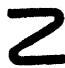
\includegraphics[keepaspectratio]{images/part002_406c0853.jpg}}

应当指出，若 \(f\) 是 \(\mathbf{Y}_1\) 到 \(\mathbf{Y}_2\) 上的双射且一致连续的映射，则它的连续延拓未必是单射，也未必是满射（习题 3）。
% semantic-fragments: legacy-input-seam
\relax{}
